% Editable native annotations around unchanged verified IDE photographs.
\par
\begin{figure}[htbp]
\centering
\newsavebox{\MARScborrecordregistersBox}
\sbox{\MARScborrecordregistersBox}{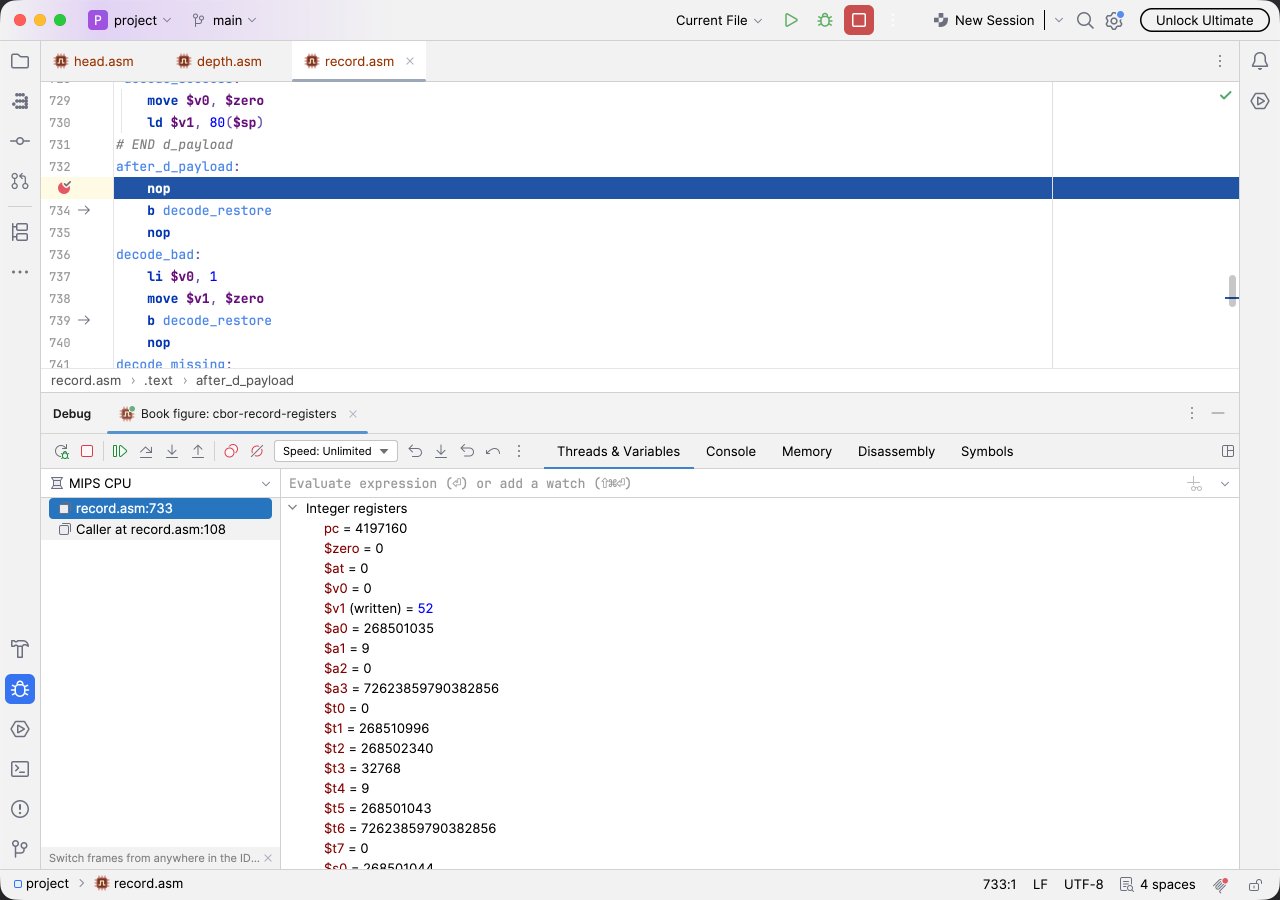
\includegraphics[artifact]{packages/032-cbor-telemetry/captures/published-record/registers.png}}
\newsavebox{\MARScborrecordprefixBox}
\sbox{\MARScborrecordprefixBox}{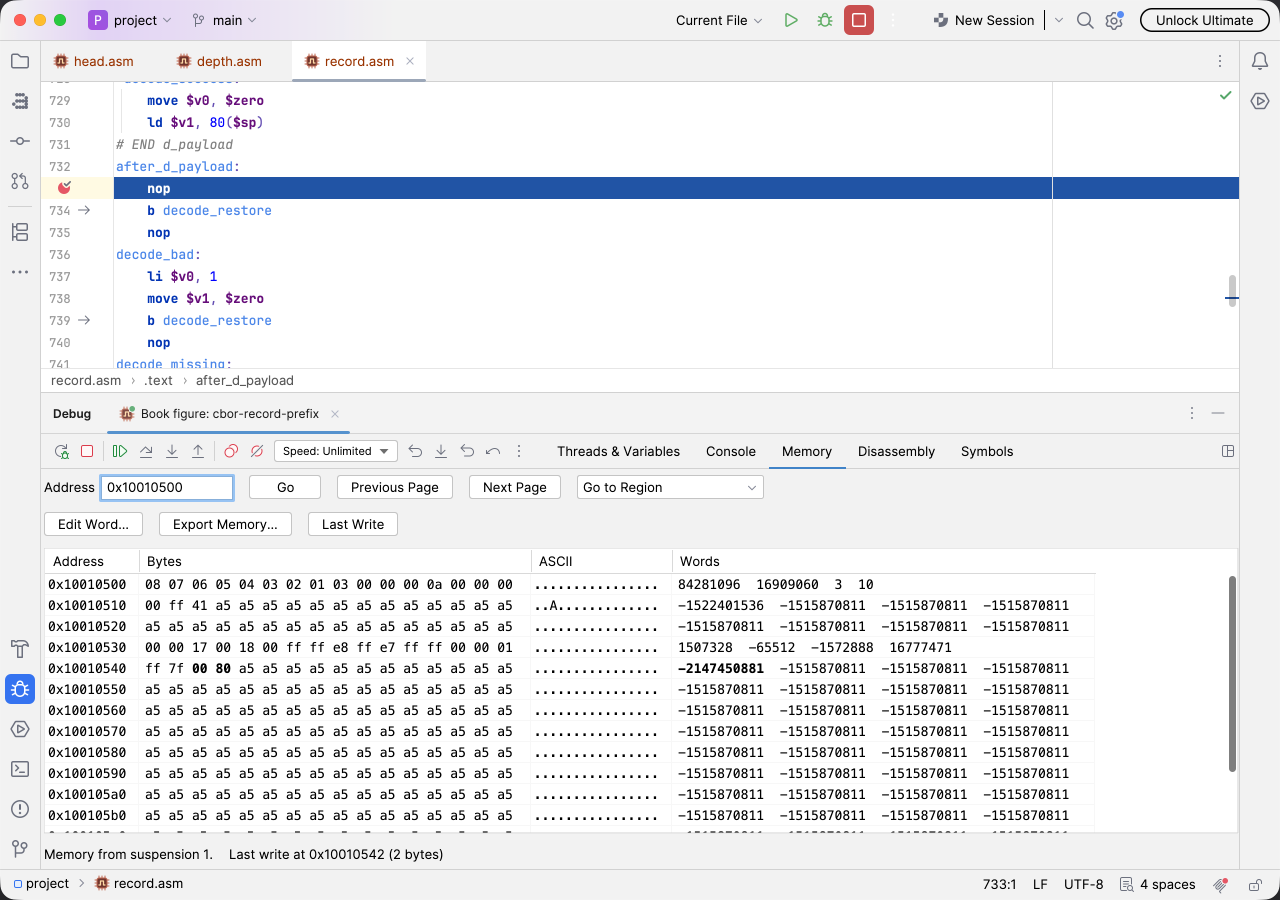
\includegraphics[artifact]{packages/032-cbor-telemetry/captures/published-record/prefix.png}}
\newsavebox{\MARScborrecordsamplesBox}
\sbox{\MARScborrecordsamplesBox}{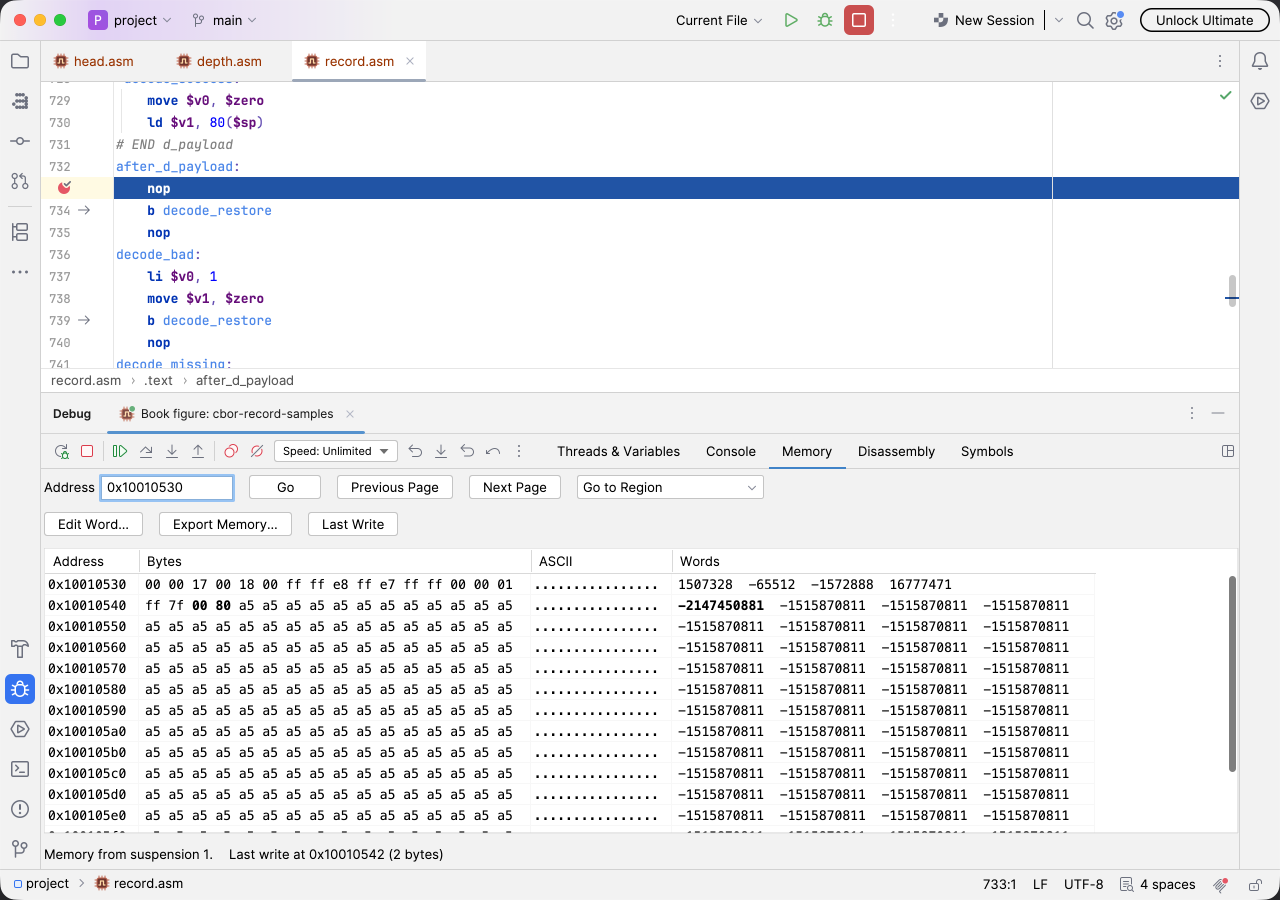
\includegraphics[artifact]{packages/032-cbor-telemetry/captures/published-record/samples.png}}
\newsavebox{\MARScborrecordtailBox}
\sbox{\MARScborrecordtailBox}{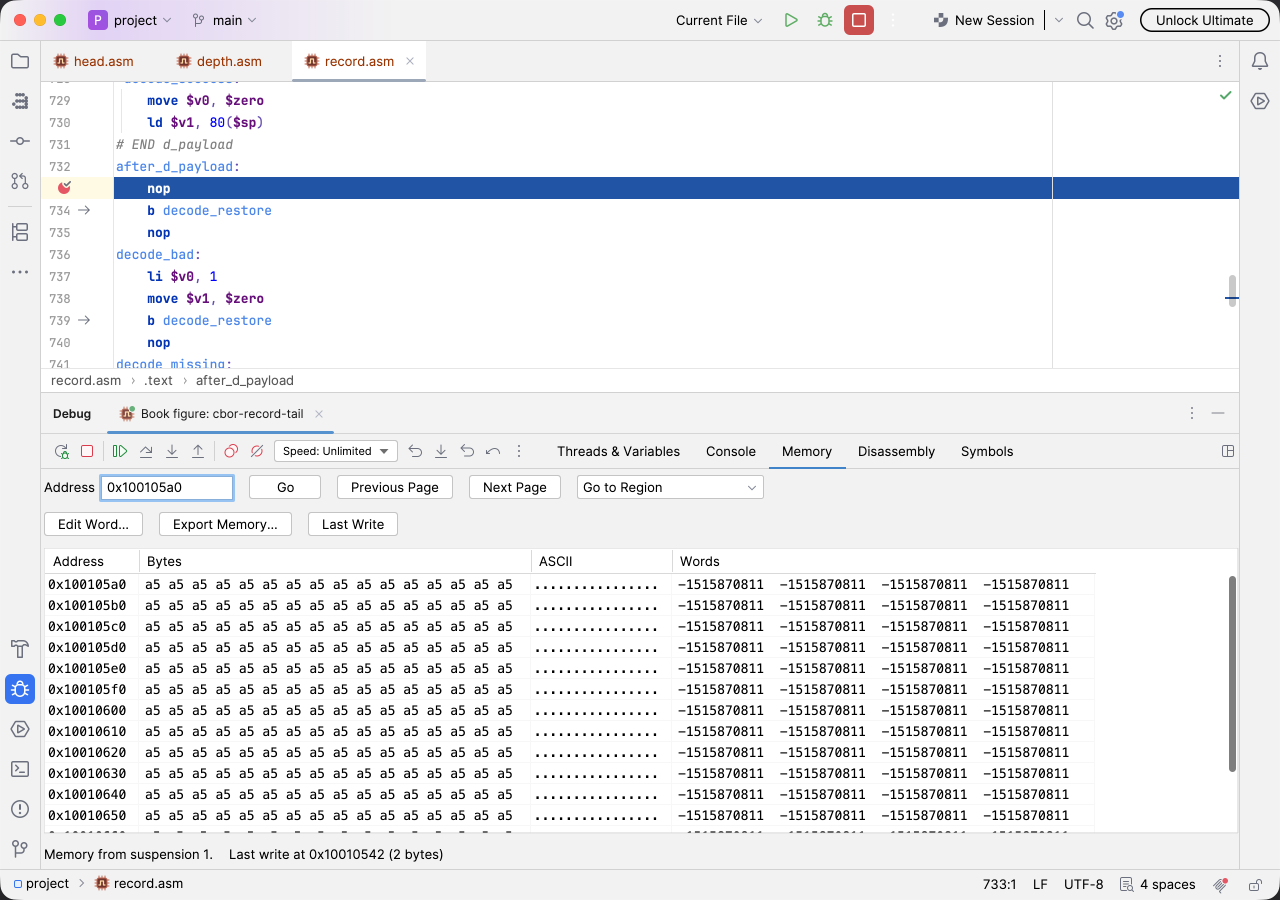
\includegraphics[artifact]{packages/032-cbor-telemetry/captures/published-record/tail.png}}
\edef\MARScborrecordsourceLeft{\the\dimexpr0.036718750\wd\MARScborrecordregistersBox\relax}
\edef\MARScborrecordsourceBottom{\the\dimexpr0.774444444\ht\MARScborrecordregistersBox\relax}
\edef\MARScborrecordsourceRight{\the\dimexpr0.713281250\wd\MARScborrecordregistersBox\relax}
\edef\MARScborrecordsourceTop{\the\dimexpr0.170000000\ht\MARScborrecordregistersBox\relax}
\edef\MARScborrecordreturnsLeft{\the\dimexpr0.246093750\wd\MARScborrecordregistersBox\relax}
\edef\MARScborrecordreturnsBottom{\the\dimexpr0.312222222\ht\MARScborrecordregistersBox\relax}
\edef\MARScborrecordreturnsRight{\the\dimexpr0.553906250\wd\MARScborrecordregistersBox\relax}
\edef\MARScborrecordreturnsTop{\the\dimexpr0.640000000\ht\MARScborrecordregistersBox\relax}
\edef\MARScborrecordprefixLeft{\the\dimexpr0.034375000\wd\MARScborrecordprefixBox\relax}
\edef\MARScborrecordprefixBottom{\the\dimexpr0.287777778\ht\MARScborrecordprefixBox\relax}
\edef\MARScborrecordprefixRight{\the\dimexpr0.584375000\wd\MARScborrecordprefixBox\relax}
\edef\MARScborrecordprefixTop{\the\dimexpr0.608888889\ht\MARScborrecordprefixBox\relax}
\edef\MARScborrecordsamplesLeft{\the\dimexpr0.034375000\wd\MARScborrecordsamplesBox\relax}
\edef\MARScborrecordsamplesBottom{\the\dimexpr0.311111111\ht\MARScborrecordsamplesBox\relax}
\edef\MARScborrecordsamplesRight{\the\dimexpr0.584375000\wd\MARScborrecordsamplesBox\relax}
\edef\MARScborrecordsamplesTop{\the\dimexpr0.608888889\ht\MARScborrecordsamplesBox\relax}
\edef\MARScborrecordtailLeft{\the\dimexpr0.034375000\wd\MARScborrecordtailBox\relax}
\edef\MARScborrecordtailBottom{\the\dimexpr0.311111111\ht\MARScborrecordtailBox\relax}
\edef\MARScborrecordtailRight{\the\dimexpr0.584375000\wd\MARScborrecordtailBox\relax}
\edef\MARScborrecordtailTop{\the\dimexpr0.608888889\ht\MARScborrecordtailBox\relax}
\begin{tikzpicture}[alt={Five details at after_d_payload show successful decoding of fifty-two bytes, the full-width little-endian counter, identifier length three and reading count ten, identifier 00 ff 41, ten signed samples, and unchanged logical and physical tails.}]
\node[anchor=north west,inner sep=0,font=\small\bfseries] (source-title) at (6mm,0) {After publishing active fields};
\node[anchor=north west,inner sep=0] (source) at ([yshift=-1mm]source-title.south west) {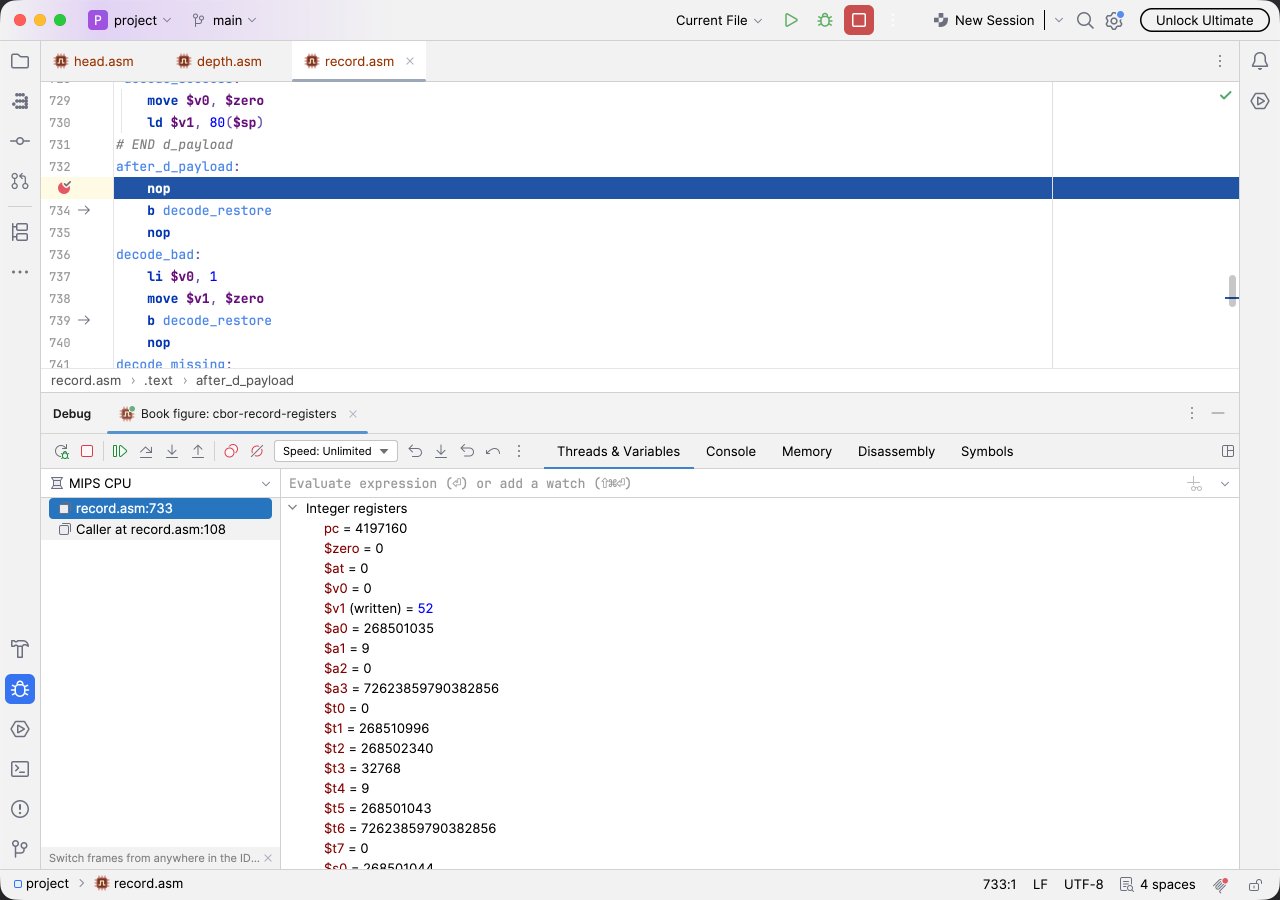
\includegraphics[width=0.54\linewidth,artifact,trim={\MARScborrecordsourceLeft{} \MARScborrecordsourceBottom{} \MARScborrecordsourceRight{} \MARScborrecordsourceTop{}},clip]{packages/032-cbor-telemetry/captures/published-record/registers.png}};
\begin{scope}[shift={(source.south west)},x={($(source.south east)-(source.south west)$)},y={($(source.north west)-(source.south west)$)}]
\draw[black,line width=0.7pt] (0.215625000,0.080000000) rectangle (0.384375000,0.520000000);
\node[draw=black,fill=white,circle,inner sep=1.5pt,font=\footnotesize] at ($(0.215625000,0.520000000)+(-3mm,0)$) {1};
\end{scope}
\node[anchor=north west,inner sep=0,font=\small\bfseries] (returns-title) at ([yshift=-1mm]source.south west) {Success and complete input length};
\node[anchor=north west,inner sep=0] (returns) at ([yshift=-1mm]returns-title.south west) {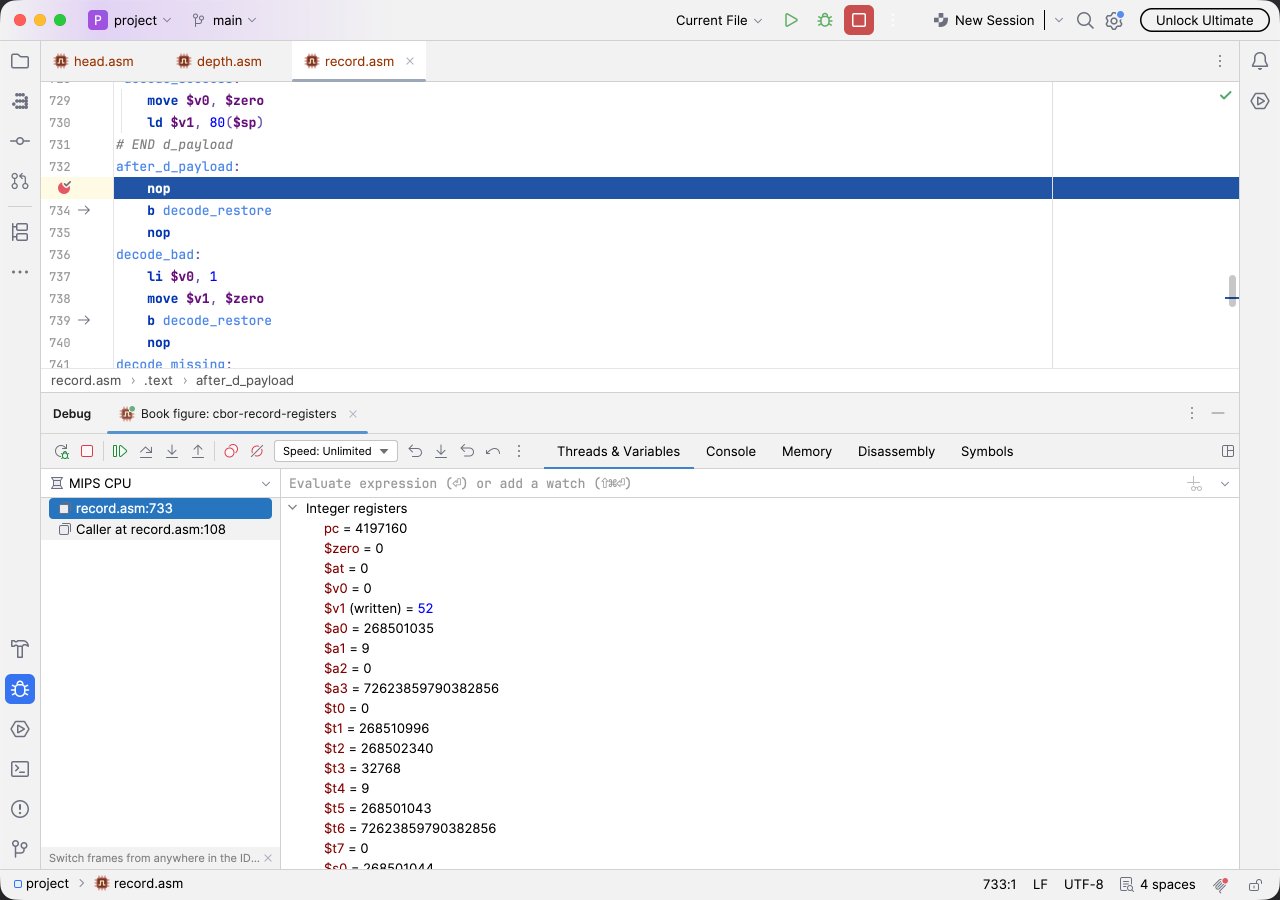
\includegraphics[width=0.48\linewidth,artifact,trim={\MARScborrecordreturnsLeft{} \MARScborrecordreturnsBottom{} \MARScborrecordreturnsRight{} \MARScborrecordreturnsTop{}},clip]{packages/032-cbor-telemetry/captures/published-record/registers.png}};
\begin{scope}[shift={(returns.south west)},x={($(returns.south east)-(returns.south west)$)},y={($(returns.north west)-(returns.south west)$)}]
\draw[black,line width=0.7pt] (0.023437500,0.023255814) rectangle (0.468750000,0.953488372);
\node[draw=black,fill=white,circle,inner sep=1.5pt,font=\footnotesize] at ($(0.023437500,0.953488372)+(-3mm,0)$) {2};
\end{scope}
\node[anchor=north west,inner sep=0,font=\small\bfseries] (prefix-title) at ([yshift=-1mm]returns.south west) {Counter, lengths and counted identifier};
\node[anchor=north west,inner sep=0] (prefix) at ([yshift=-1mm]prefix-title.south west) {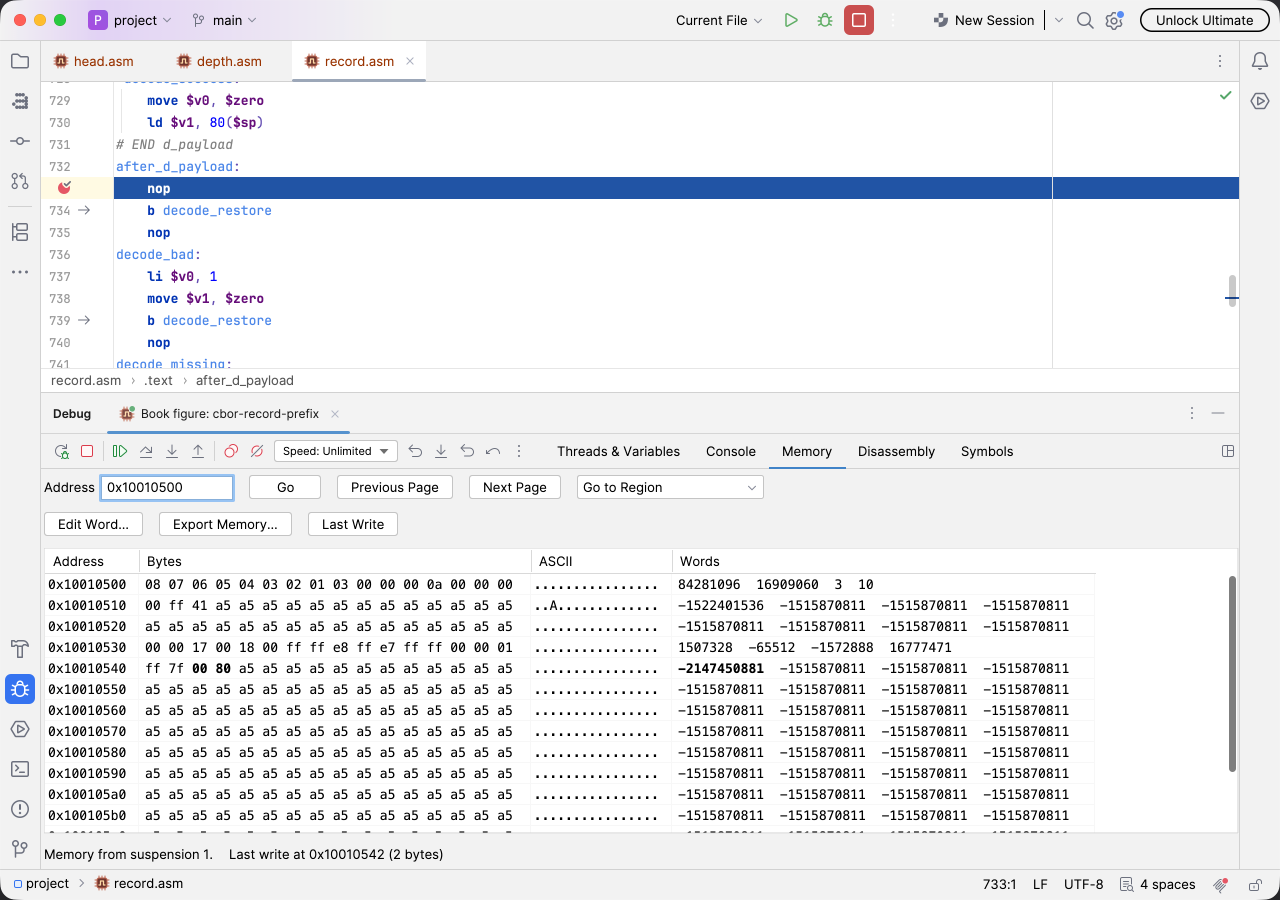
\includegraphics[width=0.84\linewidth,artifact,trim={\MARScborrecordprefixLeft{} \MARScborrecordprefixBottom{} \MARScborrecordprefixRight{} \MARScborrecordprefixTop{}},clip]{packages/032-cbor-telemetry/captures/published-record/prefix.png}};
\begin{scope}[shift={(prefix.south west)},x={($(prefix.south east)-(prefix.south west)$)},y={($(prefix.north west)-(prefix.south west)$)}]
\draw[black,line width=0.7pt] (0.194672131,0.043010753) rectangle (0.997950820,0.720430108);
\node[draw=black,fill=white,circle,inner sep=1.5pt,font=\footnotesize] at ($(0,0.720430108)+(-3mm,0)$) {3};
\end{scope}
\node[anchor=north west,inner sep=0,font=\small\bfseries] (samples-title) at ([yshift=-1mm]prefix.south west) {Ten readings followed by inactive slots};
\node[anchor=north west,inner sep=0] (samples) at ([yshift=-1mm]samples-title.south west) {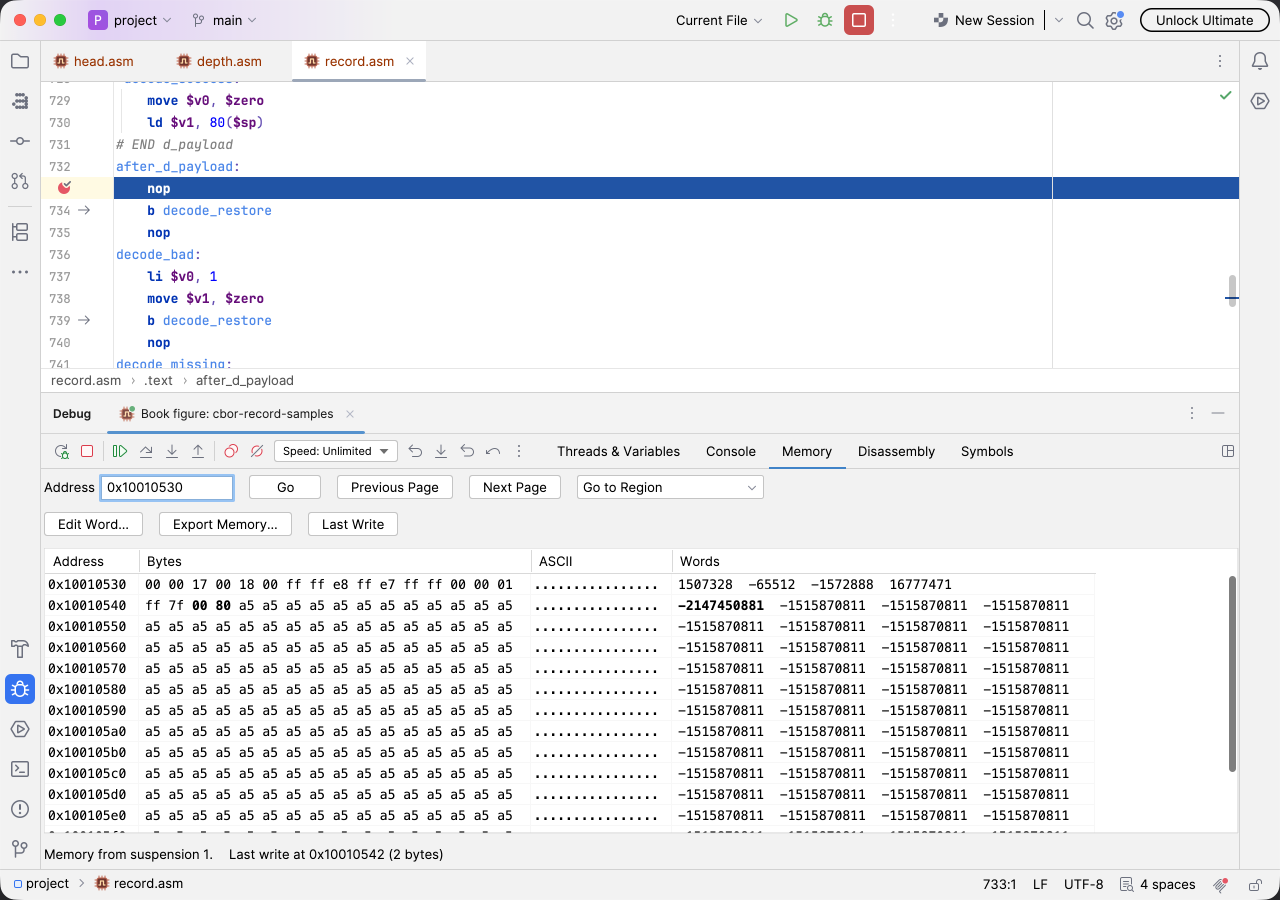
\includegraphics[width=0.84\linewidth,artifact,trim={\MARScborrecordsamplesLeft{} \MARScborrecordsamplesBottom{} \MARScborrecordsamplesRight{} \MARScborrecordsamplesTop{}},clip]{packages/032-cbor-telemetry/captures/published-record/samples.png}};
\begin{scope}[shift={(samples.south west)},x={($(samples.south east)-(samples.south west)$)},y={($(samples.north west)-(samples.south west)$)}]
\draw[black,line width=0.7pt] (0.194672131,0.055555556) rectangle (0.997950820,0.638888889);
\node[draw=black,fill=white,circle,inner sep=1.5pt,font=\footnotesize] at ($(0,0.638888889)+(-3mm,0)$) {4};
\end{scope}
\node[anchor=north west,inner sep=0,font=\small\bfseries] (tail-title) at ([yshift=-1mm]samples.south west) {Logical tail and backing suffix};
\node[anchor=north west,inner sep=0] (tail) at ([yshift=-1mm]tail-title.south west) {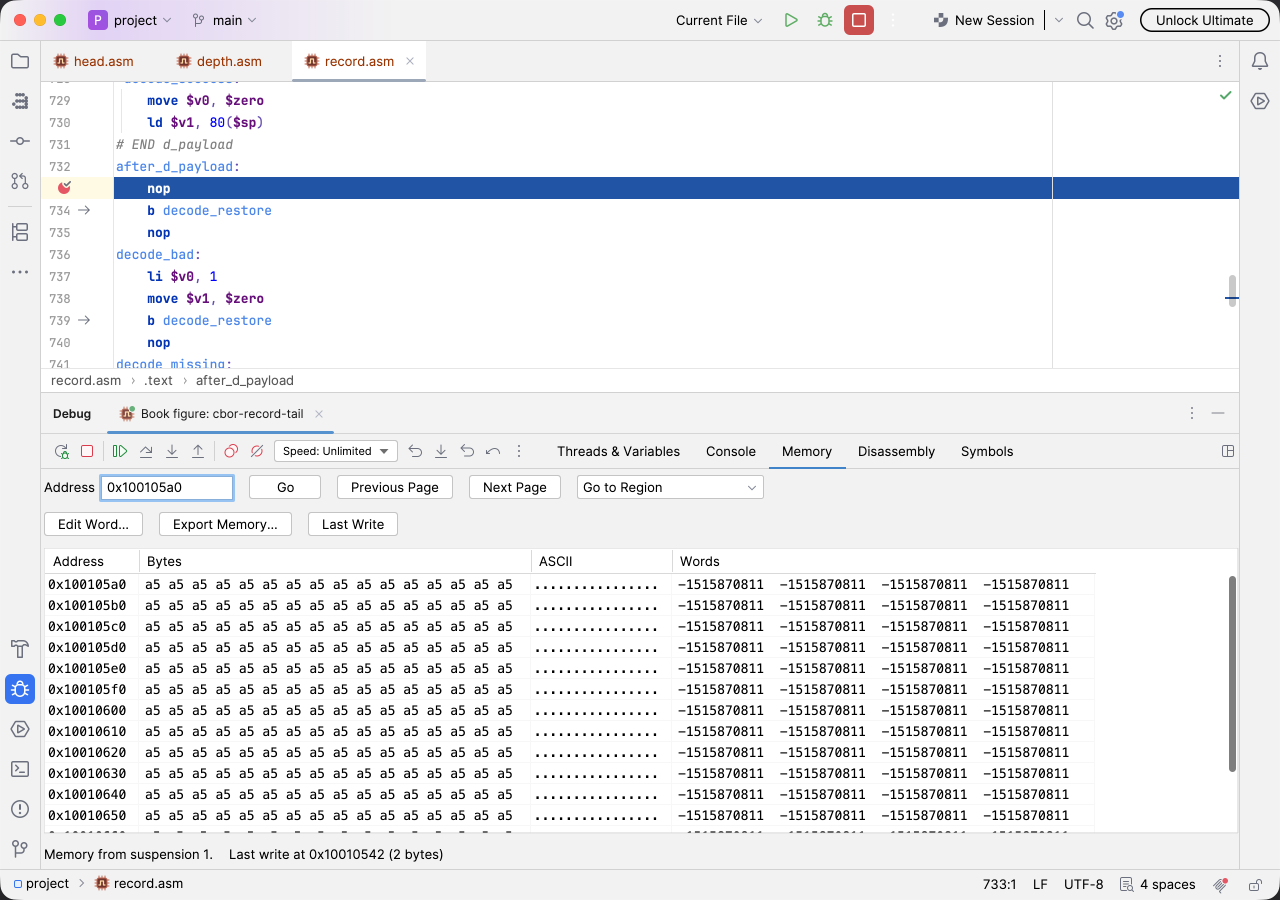
\includegraphics[width=0.84\linewidth,artifact,trim={\MARScborrecordtailLeft{} \MARScborrecordtailBottom{} \MARScborrecordtailRight{} \MARScborrecordtailTop{}},clip]{packages/032-cbor-telemetry/captures/published-record/tail.png}};
\begin{scope}[shift={(tail.south west)},x={($(tail.south east)-(tail.south west)$)},y={($(tail.north west)-(tail.south west)$)}]
\draw[black,line width=0.7pt] (0.194672131,0.055555556) rectangle (0.997950820,0.638888889);
\node[draw=black,fill=white,circle,inner sep=1.5pt,font=\footnotesize] at ($(0,0.638888889)+(-3mm,0)$) {5};
\end{scope}
\end{tikzpicture}
\par\smallskip
\begin{minipage}{\linewidth}
\small
\begin{enumerate}
\setlength{\itemsep}{0pt}
\setlength{\parsep}{0pt}
\item At \texttt{after\_d\_payload}, publication has completed but the decoder has not yet restored its frame. The selected \texttt{nop} is an observation boundary before \texttt{decode\_restore}.
\item \texttt{v0 = 0} reports success and \texttt{v1 = 52} is the complete selected input length. It is not the flat record size or the encoded output size computed later.
\item The first eight bytes store counter \texttt{0x0102030405060708} low byte first. The next two four-byte fields hold identifier length three and sample count ten. At offset sixteen, \texttt{00 ff 41} is a counted binary identifier: the first zero byte does not terminate it. Its remaining allocated bytes retain \texttt{a5}.
\item Ten little-endian signed halfwords occupy record offsets forty-eight through sixty-seven: $0$, $23$, $24$, $-1$, $-24$, $-25$, $255$, $256$, $32767$ and $-32768$. Bytes from offset sixty-eight onward remain \texttt{a5}; publication does not clear unused sample slots.
\item The row at record offset 160 is still inside the 176-byte logical record. The next row, at offset 176, is backing storage beyond that object. Both remain unchanged. The independent checks compare the complete 256-byte caller arena, including its inactive fields and backing suffix.
\end{enumerate}
\end{minipage}
\caption{Successful decoding publishes active fields while preserving their unused tails.}
\label{capture:032-cbor-telemetry-published-record}
\label{cbor-published-record}
\end{figure}
\par
